\chapter{User Manual \label{chap:usermanual}}
The system is designed to be cross platform, however it is advised to use Windows as it is the only system on which the project was thoroughly tested.

\section{Requirements and installation \label{sec:requirements}}
Before using the software, several requirements must be fulfilled.

\subsection{Software and Libraries}
\subsubsection{Required software}
\smallskip
\begin{itemize}
	\item Python 2.7
	\item Pip
	\item Blender version 2.79 or newer\footnote{Blender can be obtained from the official Blender website:  \url{http://www.blender.org/}}
\end{itemize}

\subsubsection{Libraries}
\smallskip
\textbf{Only for Linux systems: Download and install library python-dev (or python-devel) before following the instructions below}

\noindent Following python libraries must be installed (using pip, easy-install, or any other python packet manager):
\begin{itemize}
	\item setuptools
	\item watson-developer-cloud
	\item wget
\end{itemize}
\noindent The packages can be installed in bulk by running:

\indent `path\_to\_python/Scripts/pip install -r requirements`

\noindent in the main directory. As Blender usually comes with its own Python environment, you will need to run the command:

\indent `path\_to\_blender/version/python/Scripts/pip install -r requirements`

\noindent To install the libraries for Blender.

\subsection{Install Generator as Blender Addon \label{sec:installaddon}}
The following steps are optional. Installing the module as addon will enable the module to be permanently incorporated into Blender.

\noindent To install the addon:
\begin{enumerate}
	\item Open Blender
	\item Open user settings (File > User preferences)
	\item Open Add-ons tab
	\item On the bottom panel press `install add-on from file`
	\item Navigate to `project folder > generator` and double click on `addon.py`
	\item In the search box on the top right corner type `NLPanim` - a greyed-out item called `Object: NLPAnim` should appear
	\item Check the box next to the item
	\item Press `Save user settings` in the bottom left corner
	\item Exit user preferences
\end{enumerate}

\noindent The module is now installed as an add-on. In the 3D-view (default view) on the bottom of the left-hand side menu there should appear a tab called `Generate NLP anim` (figure ~\ref{fig:installedaddon}).
	
\begin{figure}[!ht]
	\centerline{\fbox{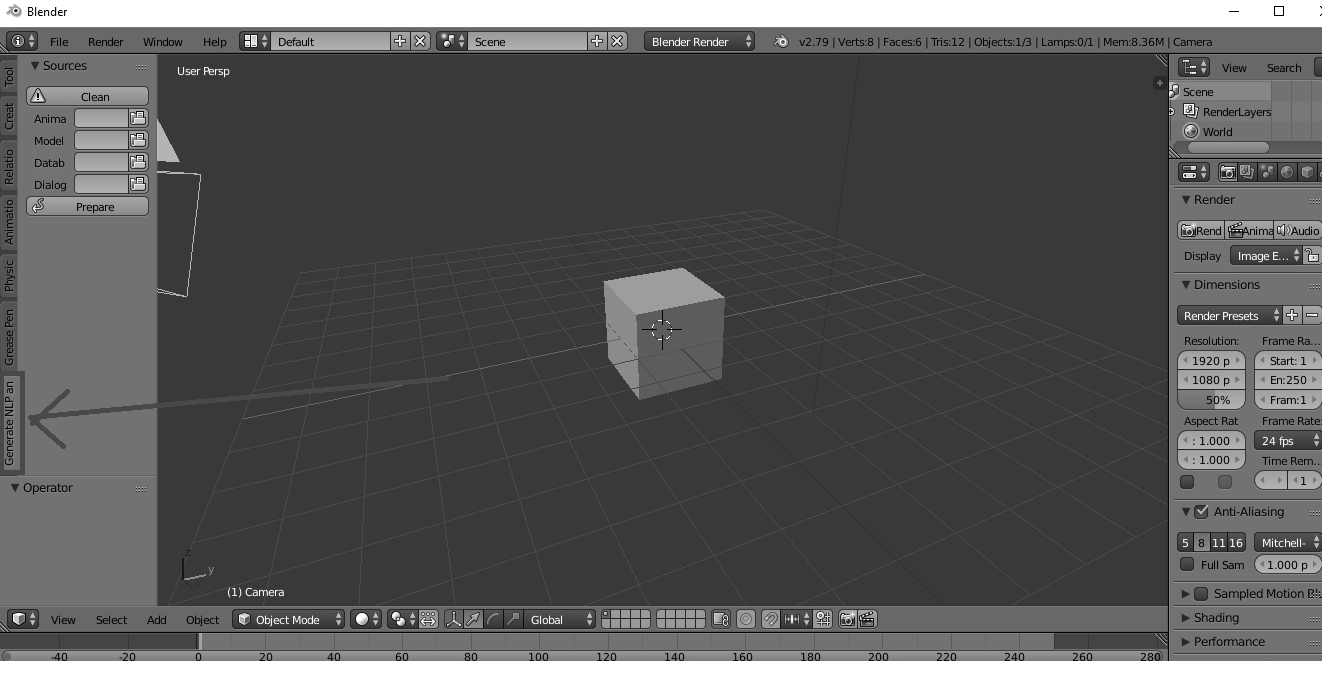
\includegraphics[width = 30em]{img/appendix/installedaddon.png}}}
	\caption{The generator addon menu}\label{fig:installedaddon}
\end{figure}

\section{Generating animations \label{sec:generatormanual}}
\noindent Now that all the requirements are met, the animation can be generated. There are two main steps to generating. Firstly, use the analyzer module to create a scene.json file\footnote{scene.json is a JSON file which contains instructions for the generator module that describe how to assemble the animation.}. Secondly, use the generator to assemble the animation.

\subsubsection{Analyze script \label{sec:analyze-script}}
\noindent The input script must resemble the script in figure ~\ref{fig:inputscript2}

\begin{figure}[!ht]
	\centerline{\fbox{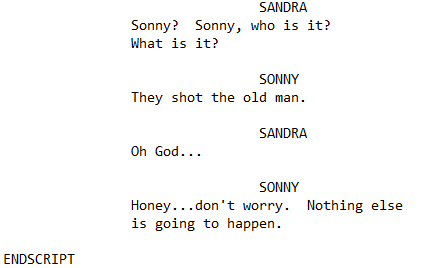
\includegraphics[width = 30em]{img/script.png}}}
	\caption{An example of system's input}\label{fig:inputscript2}
\end{figure}

\noindent The characters must be specified after 5 tabs. The dialogue text is specified after 3 tabs. The file must end with an `ENDSCRIPT` with no indentation. For reference please refer to either:
\begin{itemize}
	\item Example script files in folder `movies`
	\item Movie scripts hosted on \url{http://www.imsdb.com}
\end{itemize}

\noindent The script now can be process using the following command:

\indent `python analyzer/script\_analyze.py path\_to\_dialogue\_script db/animation.db`

\noindent The program will output a file called `scene.json`. This file is used to generate the animation.

\subsubsection{Generate Animation}
\noindent If you did not install the module as a Blender add-on (if you skipped section ~\ref{sec:installaddon}), please follow these steps:
\begin{enumerate}
	\item Open the file `rendered.blend` with Blender
	\item Click `Run Script` on the bottom of the scripting view (figure ~\ref{fig:withoutaddon})
	\item The tab called `Generate NLP anim` should appear on the right hand side menu of the 3D view
	\item Click on the `Generate NLP anim` tab
\end{enumerate}

\begin{figure}[H]
	\centerline{\fbox{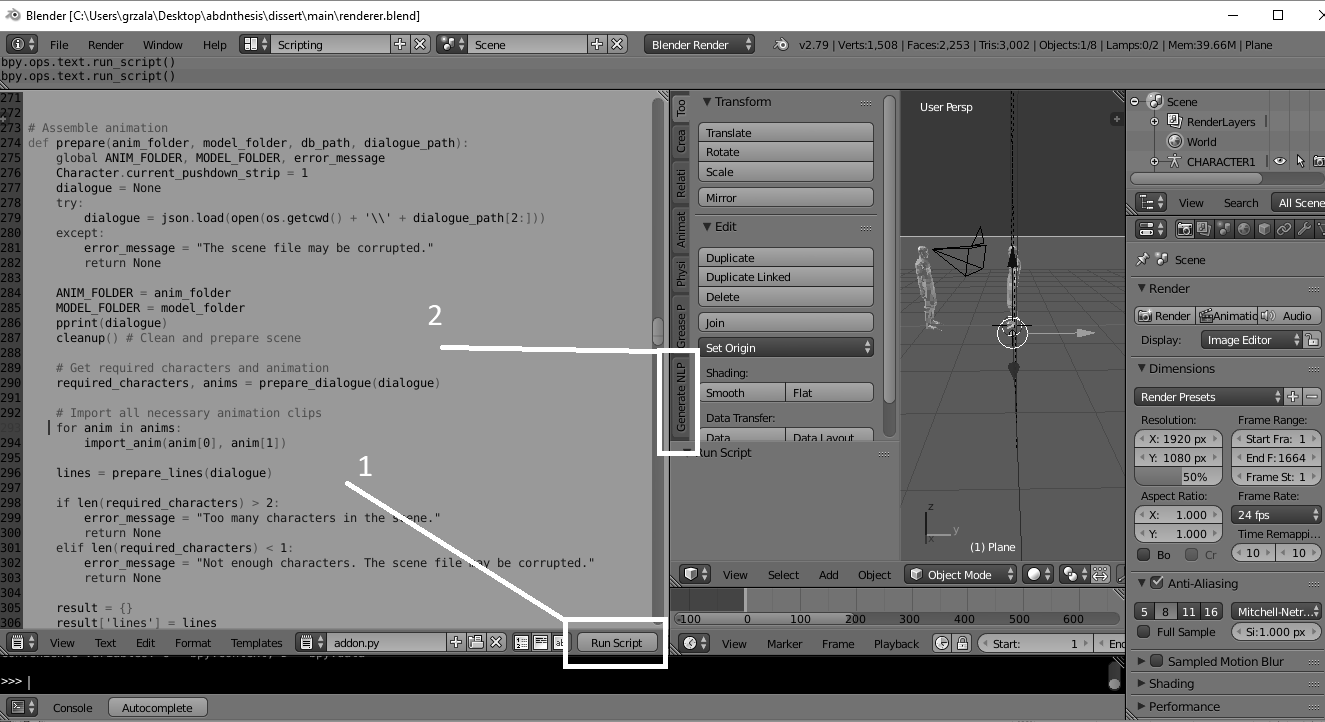
\includegraphics[width = 30em]{img/appendix/withoutaddon.png}}}
	\caption{Running the generator without installing it as an add-on}\label{fig:withoutaddon}
\end{figure}

Please follow these steps only if you installed the generator as an add-on:
\begin{itemize}
	\item Open Blender
	\item Press `File > Save` and save the file in a preferred location
	\item \textbf{Important:} close Blender and reopen the saved file
	\item Open `Generate NLP anim` tab
\end{itemize}

\noindent After finishing the above instructions, do the following to finalize the animation:
\begin{enumerate}
	\item Press `Clean` at the top of the menu
	\item Choose the directory `mocap` for `Animations Directory`
	\item Choose the directory `models` for `Models Directory`
	\item Choose the file `db/animation.db` for `Database`
	\item For `Dialogue` choose the `scene.json` file you created when following the section ~\ref{sec:analyze-script}
	\item Press `Prepare` and wait until a `Finalize` menu appears below the `Prepare` button
	\item Assign models for the characters from the drop-down lists
	\item Press `Assemble` and wait until done
\end{enumerate}

\noindent The animation is now finalized. It can now be viewed, edited or rendered. Please refer to Blender official documentation and tutorials for more information on this.

\section{Using Custom Animation and Models}
This section describes how to extend or replace the animation database.

To insert a new animation file, ensure that the file is saved as .fbx file and contains only one animation (action). Please make sure that the armature\footnote{Armature is a skeleton; A set of bones that can be animated. If you are unsure of what an armature is, you should avoid using custom animations and models.} is compatible with the one found in `EMBD importer/armature.fbx` file.

To continue you will need to install `DB Browser for Sqlite`\footnote{The DB browser for Sqlite can be obtained from the sqlitebrowser official website:  \url{http://www.sqlitebrowser.org}}. Use that program to open the file `db/animation.db`. Browse the table `animations` and add a new record. Provide a name for the animation file (please note the names must be unique) and a path to the animation file. You must also fill the emotion values for the animation (set to 0.0 if the emotion is not carried by the animation).

To insert a new model, browse the `models` table. Again, provide a unique name and a file path for the .fbx model. You will also need to provide information on how to position and rotate the camera to focus it on the characters face (relative to the origin of the character model\footnote{The origin of a character model is usually a point on the floor between the character's feet (directly below the spine).}). You will need to provide six values in total.
\begin{itemize}
	\item Offset on axis X, Y and Z (positive Z means upwards, negative Y is forwards and positive X is to the right) in Blender units (distance).
	\item Rotation on axis X, Y and Z in degrees.
\end{itemize}

\noindent You can use your own database file as long as the database keeps the following structure:
\begin{itemize}
	\item `animations` table:
	
	\begin{itemize}
		\item id (Integer, unique, primary key)
		\item name (Text, unique)
		\item file (Text)
		\item Frames (Integer)
		\item anger (Numeric)
		\item joy (Numeric)
		\item sadness (Numeric)
		\item fear (Numeric)
		\item disgust (Numeric)
		\item surprise (Numeric)
	\end{itemize}

	\item `models` table:
	
	\begin{itemize}
		\item ID (Integer, unique, primary key)
		\item name (Text, unique)
		\item file (Text)
		\item cam\_offset\_x (Numeric)
		\item cam\_offset\_y (Numeric)
		\item cam\_offset\_z (Numeric)
		\item cam\_rot\_x (Numeric)
		\item cam\_rot\_y (Numeric)
		\item cam\_rot\_z (Numeric)
	\end{itemize}
\end{itemize}

\noindent Keep the emotion values from 0.0 to 1.0.


\section{Importing More Animations From EMBD}
If you wish to import more animations from EMBD you can use the EMBD importer tool. It will allow you to quickly process huge amounts of EMBD animations and export them to .fbx files compatible with the project.

\noindent To use the importer tool
\begin{enumerate}
	\item Open file `EMBD importer/importer.blend` with Blender
	\item In the text editor on the left scroll to the bottom
	\item There you will find arrays with links to EMBD animations
	\item Visit \url{http://ebmdb.tuebingen.mpg.de/index.php}
	\item Browse the EMBD website in search of desired animations
	\item Copy the links to BVH files and paste them in the arrays in the script
	\item Press `Run Script` on the bottom panel
	\item \textbf{Important:} The process might take a long time depending on the amount of required animations - please do not interrupt or close Blender even when the system labels the process as unresponsive
	\item The imported files can be found in the folder `imported`
\end{enumerate}


\section{Generate a Showcase \label{sec:showcasegeneratormanual}}
Since all animations must be reviewed manually in order to assign their emotion value the showcase generator tool was created to help with this task. The process of generating a showcase will take a number of animations and display them all in one animated clip while showing their filenames as subtitles

\noindent To generate a showcase:
\begin{enumerate}
	\item Run the command `python analyzer/generate\_showcase.py path\_to\_directory\_with\_animations`
	\item The program will create a number of json files (showcase0.json, showcase1.json, etc) in the `showcases` folder
	\item Each showcase file contains instructions for the generate to create an animation consisting of up to 10 animation (splitting the scene into 10 clips each makes it easier to render and use)
	\item Use the showcase files as scene files with the generator module (section ~\ref{sec:generatormanual})
	\item Render the animation
\end{enumerate}


